\documentclass[12pt]{fithesis2}

% ===== LOADING PACKAGES =====
% language settings, main documnet language last
\usepackage[english]{babel}
% enabling new fonts support (nicer)
\usepackage{lmodern}
% setting input encoding
\usepackage[utf8]{inputenc}
% setting output encoding
\usepackage[T1]{fontenc}
% fithesis2 requires csquotes
\usepackage{csquotes}

\usepackage{subfig}
\usepackage{graphicx}
\usepackage{kpfonts}
\usepackage[labelfont=bf]{caption}
\usepackage{stmaryrd}
\usepackage{mathtools}
\usepackage[usenames, dvipsnames]{color}
\usepackage{esvect}

\newcounter{counter}[section]
\renewcommand{\thecounter}{\thesection.\arabic{counter}}
\newcommand{\definition}[1]{\refstepcounter{counter} \textbf{Definition \thecounter} \newline #1 }
\newcommand{\notation}[1]{\refstepcounter{counter} \textbf{Notation \thecounter} \newline #1 }
\newcommand{\theorem}[1]{\refstepcounter{counter} \textbf{Theorem \thecounter} \newline #1 }
\newcommand{\example}[1]{\refstepcounter{counter} \textbf{Example \thecounter} \newline #1 }
\newcommand{\runningExample}[1]{\refstepcounter{counter} \textbf{Running Example \thecounter} \newline #1 }

\usepackage[
    backend=biber,      % use biber as backend instead of BiBTeX
    style=alphabetic,   % citation style
	url=true,           % display urls in bibliography
	hyperref=auto,      % detect hyperref and create links
    firstinits=true,    % abbreviate first names to initials
    maxbibnames=5,      % maxiumim number of authors before making 'et al.'
    alldates=iso8601,   % set date format to ISO 8601
]{biblatex}
\addbibresource{thesis.bib}
% setting custom colors for l

% FI THESIS settings
\thesistitle{Something with BCS}
\thesissubtitle{Master thesis}
\thesisstudent{Matej Troják}
\thesiswoman{false}
\thesisfaculty{fi}
\thesisyear{autumn 2017}
\thesisadvisor{RNDr.\ David Šafránek,\ Ph.D.}
\thesislang{en}

% ===== BEGIN DOCUMENT =====
\begin{document}

\FrontMatter
\ThesisTitlePage

\begin{ThesisDeclaration}
\DeclarationText
\AdvisorName
\end{ThesisDeclaration}

\begin{ThesisThanks}
Many thanks to you all.

\vspace{1em}
\noindent
There would be much less
algebra,        % advancements, art, adrenaline, archery, astrophotography, algebra
board gaming,   % beauty, baking, beer, board gaming
curiosity,      % courage, contemplation, cooking, cakes, curiosity
drama,          % discipline, devotion, drama
experience,     % empathy, experience
functional programmig,  % fun, friendliness, faith, functional programmig
geekiness,      % GEB, good books, geekiness
honesty,        % humour, honesty
inspiration,    % improvements, ideas, idealisms, inspiration
joy,            % jokes, joy
knowledge,      % knowledge
learning,       % learning, love
magic,          % meaning, magic, miracles, meta, moose
nighttime walks,    % nighttime walks, Norway
OpenLabs,       % organization, openness, optimism, OpenLabs
puzzle hunts,   % peace, patience, procrastination, puzzle hunts
quiet,          % quiet
respect,        % research, respect
surprises,      % spontaneity, silence, security, stories, star gazing, surprises
trust,          % typographic correctness, tolerance, trust
unpredictability,   % understanding, unity, unpredictability
vigilance,      % vigilance
Wachumba,       % wisdom, Wachumba
xylophone,      % xylophone
yummies         % yellow, you, yummies
and
zeal            % Zendo, Zen, zeal
in the world for me without you.

\vspace{0.65\textheight}
\noindent
Access to computing and storage facilities owned by parties and projects contributing to the National Grid Infrastructure MetaCentrum, provided under the programme Projects of Large Infrastructure for Research, Development, and Innovations(LM2010005), is greatly appreciated.
\end{ThesisThanks}

\begin{ThesisAbstract}
This thesis explores the randomness of outputs created by authenticated encryption schemes submitted to the  competition. Tested scenarios included three different modes of public message numbers. For the assessment, four different software tools were used: three common statistical batteries and a novel genetically inspired framework. The obtained results are interpreted in two ways: Firstly, to gain insights into the quality of the proposed  candidates. Secondly, to compare and contrast the used randomness testing tools. Directions for future research are proposed based on the obtained conclusions.
\end{ThesisAbstract}

\begin{ThesisKeyWords}
statistical randomness, authenticated encryption, CAESAR, evolutionary algorithms, genetic programming
\end{ThesisKeyWords}

\MainMatter
\tableofcontents

\chapter{Introduction}

\chapter{Background}
\section{Rule-based basics}
\label{Rule-based basics}

In our last paper~\cite{Ded201627}, we defined semantics of Biochemical Space Language (BCSL) via translating to a similar language called Kappa~\cite{Kappa}. However, we realised this approach is not very beneficial since we are not fully using the expressive power of our language this way. The thing is Kappa operates purely on expressions. We want to promote our language to a higher level when it operates on objects in multisets. By translating to Kappa we loose such abstraction. 

The reason for this kind of abstraction is the way how we see the biological models. We represent model $\mathcal{M}$ as set of rules and an initial solution of interacting entities. We understand solution as a mixture of individual objects which are randomly distributed (see Fig.~\ref{solutions:fig}a). Therefore, we cannot assign them any order and we do not see them as expressions but rather as multisets. For us, this representation of solution is the closest to the reality.

\begin{figure}
\begin{center}
\subfloat[]{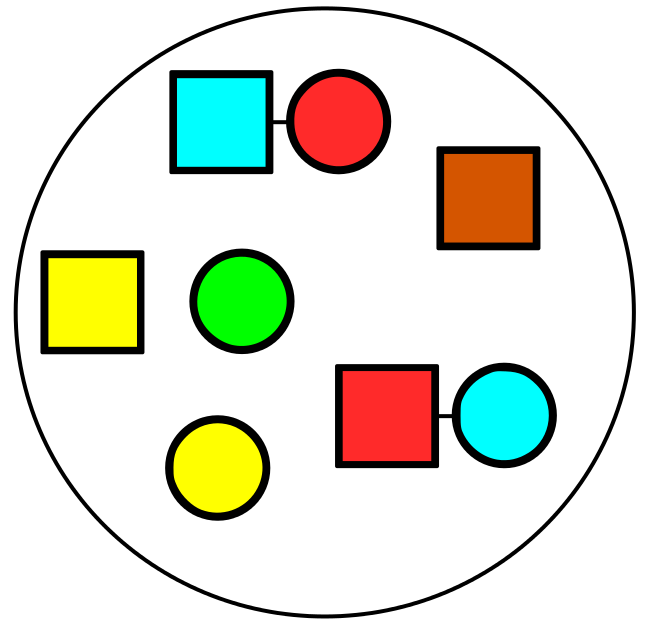
\includegraphics[scale=0.23]{solution_first}\label{sol:s1}}
\hspace*{1cm}
\subfloat[]{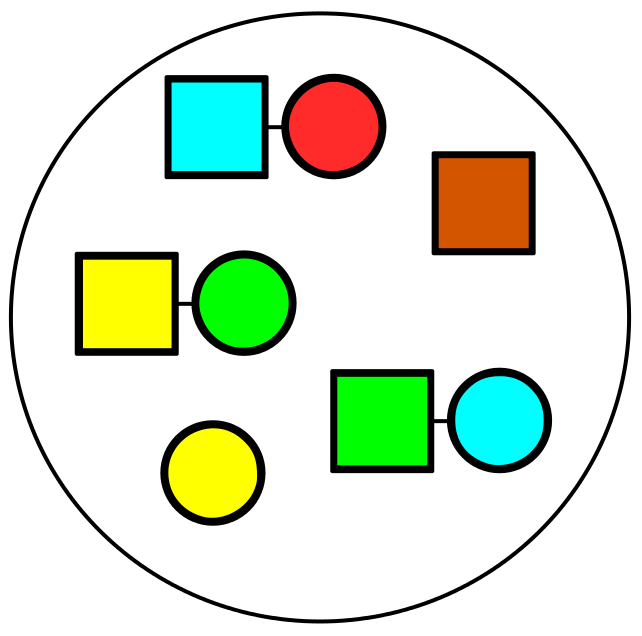
\includegraphics[scale=0.23]{solution_second}\label{sol:s2}}
\caption{\textbf{Examples of solutions}. \textbf{(a)} An example of graphical representation of a solution. \textbf{(b)} Updated solution after rules from Fig.~\ref{rules:fig} were applied. The first rule \textit{(a)} was applied on the yellow $\square$ and green $\bigcirc$ and produced yellow-green complex $\square$--$\bigcirc$. Note there are more options how the rule could be mapped -- each combination of free $\square$ and $\bigcirc$. The second rule \textit{(b)} was applied on red-cyan complex $\square$--$\bigcirc$ where the color of $\square$ was changed from red to green. The third rule \textit{(c)} couldn't be applied because there is no such complex with yellow $\bigcirc$. }
\label{solutions:fig}
\end{center}
\end{figure}

On the other hand, the rules are expressions which describe behaviour of groups of objects. A rule has form of a chemical reaction, where substrates and products take place. The difference is that reaction only operates on particular objects. Therefore, a reaction can be seen as a special case of rule (see Fig.~\ref{rules:fig}), where the groups contain exactly one element.

The rule can be mapped on a solution. Then, if it is mapped, it can be applied and a new solution is produced. The mapping is not always successful (see Fig.~\ref{solutions:fig}, application of rule \textit{c}). By repeating map-apply action, we obtain a \textit{Labelled transition system} $\mathcal{L}$.

\begin{def}\label{lts}
\textit{Labelled transition system} (LTS) $\mathcal{L}$ is a tuple $(S, A, \Delta, s_0)$ where:
\begin{itemize}
	\item $S$ is a (potentially infinite) set of states (solutions)
	\item $A$ is a set of labels (reactions)
	\item $\Delta \subseteq S \times A \times S$ is a transition relation (the map-apply action)
	\item $s_0 \in S$ is the initial state (initial solution)
\end{itemize}
\end{def}

\begin{figure}[!h]
\begin{center}
\begin{minipage}[l]{0.1\textwidth}
    \textbf{(a)}
  \end{minipage}
  \begin{minipage}[r]{0.6\textwidth}
    {\hspace*{0.8cm}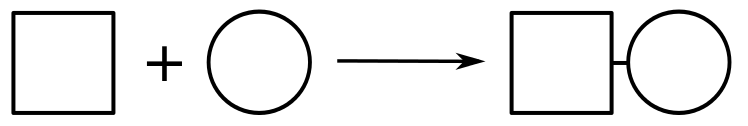
\includegraphics[scale=0.2]{rule_complex}}
\end{minipage}

\begin{minipage}[l]{0.1\textwidth}
    \textbf{(b)}
  \end{minipage}
  \begin{minipage}[r]{0.6\textwidth}
    {\hspace*{1.35cm}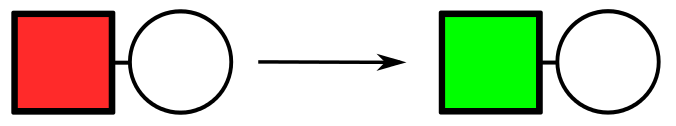
\includegraphics[scale=0.2]{rule_change}}
\end{minipage}

\begin{minipage}[l]{0.1\textwidth}
    \textbf{(c)}
  \end{minipage}
  \begin{minipage}[r]{0.6\textwidth}
    {\hspace*{1.3cm}
\includegraphics[scale=0.2]{rule_diss}}
\end{minipage}
\caption{\textbf{Examples of rules}. Rule \textbf{(a)}: a $\square$ and a $\bigcirc$ can form a complex $\square$--$\bigcirc$ regardless their colors. Rule \textbf{(b)}: a $\square$ is allowed to change it's color from red to green only if it formed a complex with a $\bigcirc$ regardless it's color. Rule \textbf{(c)}: the rule can disassemble the complex only if the $\bigcirc$ is yellow.}
\label{rules:fig}
\end{center}
\end{figure}

The mapping of a rule on a solution can be seen as a particular moment, when the objects in the solution have just the conformation suitable for the rule and therefore the rule can be applied. However, since the distribution of objects is random, we can assume a sequence of objects needed for rule (if there are such objects) is always available.

Moreover, the mapping can be seen as assigning particular objects from the solution to objects on the left-hand-side of the rule. The rule application can be seen as changing the mapped objects to new objects according to the right-hand-side of the rule (i.e., particular objects are assigned to the right-hand-side). As a by-product, we obtain an instance of the rule -- a reaction (see Fig.~\ref{map-apply:fig}). This is how we construct the set of reactions $A$ in the LTS $\mathcal{L}$.

\begin{figure}
\begin{center}
\begin{minipage}[l]{0.1\textwidth}
    \textbf{(a)}
  \end{minipage}
  \begin{minipage}[r]{0.6\textwidth}
    {\hspace*{1.3cm}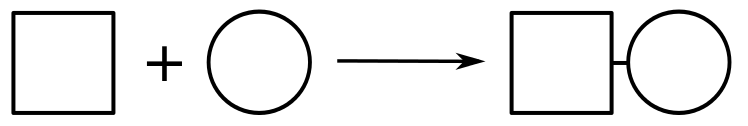
\includegraphics[scale=0.2]{rule_complex}}
\end{minipage}

\begin{minipage}[l]{0.1\textwidth}
    \textbf{(b)}
  \end{minipage}
  \begin{minipage}[r]{0.6\textwidth}
    {\hspace*{1.3cm}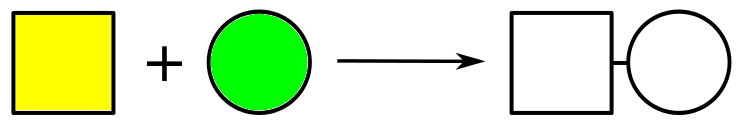
\includegraphics[scale=0.2]{rule_complex_mapped}}
\end{minipage}

\begin{minipage}[l]{0.1\textwidth}
    \textbf{(c)}
  \end{minipage}
  \begin{minipage}[r]{0.6\textwidth}
    {\hspace*{1.3cm}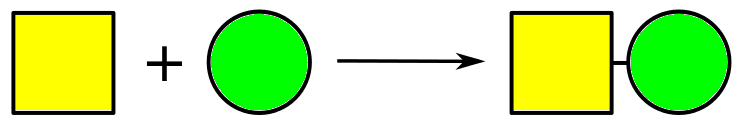
\includegraphics[scale=0.2]{rule_reaction}}
\end{minipage}
\caption{\textbf{Example of a map-apply action}. As a solution, we use solution \textit{(a)} from Fig.~\ref{solutions:fig}. \textbf{(a)} Rule can be mapped on a $\square$ and a $\bigcirc$ regardless their colors and form a complex $\square$--$\bigcirc$.  \textbf{(b)} Let's choose yellow $\square$ and green $\bigcirc$ from our solution. The rule was mapped on choosen objects and they were assigned to the left-hand-side of the rule. \textbf{(c)} The rule was applied and new object (yellow-green complex $\square$--$\bigcirc$) was created. We obtained the reaction describing the particular action which has just happened.}
\label{map-apply:fig}
\end{center}
\end{figure}

Since this kind of graphical representation is not very suitable for describing the processes and for transferring them.. ???, in next chapter(s) we define a formal language which is built on principles described in this chapter.

\section{Rule-based languages}

There are several rule-based languages dedicated for modeling of biological systems. Each of them uses different features and abstractions. In this chapter, we will try to highlight the key features for some representatives of them.

\subsection{Kappa}
\label{kappa}

This language was developed for modeling of protein-protein interactions. Therefore, the key feature of the language are it's so called \textit{agents} with \textit{binding sites}, which allow formation of bonds between the agents. Each binding site must be unique and at most one bond. Moreover, each site can occur in one of several pre-defined states.

The \textit{Kappa rules} are changing properties of the agents. Particularly, it might add/delete/change a bond or a state of one or multiple agents at once. Such as all the other rule-based languages, when we do not care about some context, we simply omit it. Example of a rule is in Figure~\ref{kappa-rule}.

\begin{figure}
\begin{center}
\begin{tabular}{c l}
(a) & A(bsa$\sim$\{ u, p \}) ; B(bsb$\sim$\{ a, i \}) \\
(b) & A(bsa), B(bsb$\sim$a) $\rightarrow$ A(bsa!1), B(bsb$\sim$a!1) \\
\end{tabular}
\end{center}
\caption{Example of a Kappa rule. (a) Definition of associated agents. (b) The rule itself. Note the context which has no importance for the interaction is omitted.}\label{kappa-rule}
\end{figure}

The general problem we have to face with in Kappa is too detailed description. For biological systems as defined in chapter~\ref{Rule-based basics}, it might be often hard to deal with all the bonds, especially in cases when we do not need such detail.

\subsection{BioNetGen Language}
\label{bngl}

BioNetGen Language (BNGL) is very similar to Kappa~\ref{kappa}. There are a few general differences: (1) it is allowed to define multiple binding sites with same name for an agent; (2) one binding site is allowed to have multiple bonds; (3) in the rules BNGL uses `+' and `.' for expressing reaction complex and complex of agents respectively. Example of a rule is in Figure~\ref{bngl-rule}.

\begin{figure}
\begin{center}
\begin{tabular}{c l}
(a) & A(bsa$\sim$u$\sim$p) \\
	& B(bsb$\sim$a$\sim$i) \\
(b) & A(bsa) + B(bsb$\sim$a) $\rightarrow$ A(bsa!1).B(bsb$\sim$a!1) \\
\end{tabular}
\end{center}
\caption{Example of a BGNL rule. (a) Definition of associated agents. (b) The rule itself. Note the A and B agents must first create \emph{reaction complex} denoted with `+' (i.e., they must be close to each other) and then they create \emph{complex of agents} denoted as `.' (i.e., they are physically connected).}\label{bngl-rule}
\end{figure}

\subsection{PySB}

This language works as a package to Python language. The definition of models directly in the code allows to use the full syntax of Python, what dramatically increases expression power of PySB. On the other hand, it might be hard to follow abstraction which are this way possible and models themselves are hard to analyze. Moreover, the core of the language is made by translating to BGNL~\ref{bngl}.

\subsection{Chromar}

The language allows to define attributes for agents and range them over pre-defined domains. The qualitative semantics are given by rule match on multisets composed from these agents producing reaction. It is followed by standard application of the reaction (in manner of multiset operations). The language is very useful when creating a model where we need to create new distinct objects and control population of these objects.

Embedding this language to functional programming language Haskell increases its expressive power while making the ability of some analysis more expensive. Moreover, one needs to learn Haskell (at least it's basics) in order to use Chromar.

\begin{figure}
\begin{center}
A(a = x), A(a = y) $\xrightarrow[]{\text{f(x,y)}}$ A(a = x + y), A(a = y - 1) [g(x, y)]
\end{center}
\caption{Example of a Chromar rule.}\label{chromar-rule}
\end{figure}

I would like to highlight an important feature of stochastic semantics which this language offers. Compared to other rule-based languages, it is capable of specifying rates for individual reactions inherited from the rule. This is allowed by variable value bindings and type-determination between left- and right-hand-side of the rule.

However, when it comes to readability and presentation to the user, the language is not a best-fit. All the biologically relevant terms such as states must be encoded to natural numbers.

\subsection{SBML-multi package}

Systems biology Markup Language (SBML) is a standard established for systems biology. It is able to describe all necessary rule-based features and therefore it is possible to export each such language in this format. It is the most suitable format for exchange and storage of the models, but less for analysis and direct representation to the users (it is and XML format). It serves as intermediate language. 

\section{Biochemical Space}

definition of BCS, what is it good for

explanation of the format, importance of annotation

from informal BCS through definition by embedding to Kappa

why not good enough

how it was evolving

what it has common with rule-based languages, how it all started

\chapter{Problem formulation}

why we need something new - need of BCS by consotium, later naturally evolved into need of formal definiton

other languages didnt use suitable level of abstraction (explain why)

what was wrong before

highlight we choose indirect definition via reactions - "practical definition"

\chapter{Formal definition}

\section{Objects definition}

Let $\mathcal{N}_{A},~\mathcal{N}_{T},~\mathcal{N}_{\delta},~\mathcal{N}_{c}$ be mutually exclusive finite sets of atomic, structure, state names, and compartments, respectively.

\begin{definition}{Signature}

\begin{itemize} 
\item Atomic signature $\Sigma_{\mathtt{A}} \subseteq \mathcal{N}_{A} \times 2^{\mathcal{N}_{\delta}}$ represents allowed atomic names with association to state names. 
\item Structure signature $\Sigma_{\mathtt{T}} \subseteq \mathcal{N}_{T} \times 2^{\mathcal{N}_{A}}$ represents allowed structure names with association to atomic names. 
\end{itemize}
\end{definition}

\begin{example}{Signature}\label{example:signature}

\begin{itemize}
\item An atomic signature $(S, \{u, p\})$, $(Q, \{a, i\})$
\item A structure signature $(KaiC, \{S, Q\})$
\end{itemize}
\end{example}

\noindent\rule{\textwidth}{1pt}

\begin{definition}{Atomic agent}

\begin{itemize}
\item Atomic agent $\mathtt{A}$ is a pair $(\mu, \delta)$ where $\mu \in \mathcal{N}_{A}$ is a name and $\delta \in \mathcal{N}_{\delta} \cup \{ \varepsilon \}$ is a state.

\item Equivalence: $\mathtt{A} \equiv \mathtt{A}' \Leftrightarrow \mu(\mathtt{A}) \equiv \mu(\mathtt{A}') \wedge \delta(\mathtt{A}) \equiv \delta(\mathtt{A}')$
\end{itemize}
\end{definition}

Note: maybe the definitino of equivalence should be done only on names (due tu partial composition in structs).

\begin{notation}
Let $\mathcal{A}$ be universe of all possible atomic agents.
\end{notation}

\begin{example}{Atomic agent}\label{example:atomic}

\begin{itemize}
\item An atomic agent $\mathtt{A}_1 = (S, u)$
\item An atomic agent $\mathtt{A}_2 = (Q, \varepsilon)$
\end{itemize}
\end{example}

Please note state $\varepsilon$ does not mean the agent is in \emph{none} state, but rather the state is unknown or not important.

\noindent\rule{\textwidth}{1pt}

\begin{definition}{Structure agent}

\begin{itemize}
\item Structure agent $\mathtt{T}$ is a pair $(\mu, \gamma)$ where $\mu \in \mathcal{N}_{T}$ is a name and $\gamma \subseteq \mathcal{A}$ is a set of atomic agents called partial composition.

\item Equivalence: $\mathtt{T} \equiv \mathtt{T}' \Leftrightarrow \mu(\mathtt{T}) \equiv \mu(\mathtt{T}') \wedge \forall \mathtt{A} \in \gamma(\mathtt{T}) \exists \mathtt{A}' \in \gamma(\mathtt{T}') : \mathtt{A} \equiv \mathtt{A}' \wedge \\ \wedge \forall \mathtt{A}' \in \gamma(\mathtt{T}') ~\exists \mathtt{A} \in \gamma(\mathtt{T}) : \mathtt{A}' \equiv \mathtt{A}$.
\end{itemize}
\end{definition}

\begin{notation}
Let $\mathcal{T}$ be universe of all possible structure agents.
\end{notation}

\begin{example}{Structure agent}\label{example:structure}

\begin{itemize}
\item A structure agent $\mathtt{T}_1 = (K, \textcolor{red}{\{}(S, p), (Q, i)\textcolor{red}{\}})$
\item A structure agent $\mathtt{T}_2 = (K, \textcolor{red}{\{}(Q, a)\textcolor{red}{\}})$
\end{itemize}
\end{example}

\noindent\rule{\textwidth}{1pt}

\begin{definition}{Complex}

\begin{itemize}
\item Complex $\mathtt{X}$ is a pair $(\mu, \mathtt{com})$ where $\mu \in (\mathcal{A} \cup \mathcal{T})^n$ is a sequence and $\mathtt{com} \in \mathcal{N}_{c}$ is a compartment.

\item Let $\mathtt{X}, \mathtt{X}'$ be complexes. We denote length of sequence $\mu$ as $n = \mu(\mathtt{X})$ and $m = \mu(\mathtt{X}')$. 

\item Equivalence: $\mathtt{X} \equiv \mathtt{X}' \Leftrightarrow n \equiv m \wedge \exists $ permutation $ \mu'(\mathtt{X}')$ of $\mu(\mathtt{X}')$ such that $\forall i~\in~[1,~n]: \mu(\mathtt{X})_i \equiv \mu'(\mathtt{X}')_i$.
\end{itemize}
\end{definition}

\begin{notation}
Let $\mathcal{X}$ be universe of all possible complexes.
\end{notation}


\begin{example}{Complex}\label{example:complex}

\begin{itemize}
\item A complex $\mathtt{X} = (\textcolor{green}{(}(K, \textcolor{red}{\{}(S, p), (Q, i)\textcolor{red}{\}}), (S, p)\textcolor{green}{)}, cytosol)$
\end{itemize}
\end{example}

\noindent\rule{\textwidth}{1pt}

\begin{definition}{Rule}

Rule $\mathtt{R}$ is a 5-tuple $(\chi, \omega, \mathtt{I}, \mathtt{map}, \mathtt{Indices})$ where:

\begin{itemize}
\item $\chi \in \mathcal{X}^n$ is a sequence of complexes,
\item $\omega \in (\mathcal{A} \cup \mathcal{T})^m$ is a sequence of atomic and structure agents,
\item $\mathtt{I} \in \{ 1, \ldots, n \}$ is an index determining start of right-hand-side,
\item $\mathtt{map} \in \mathbb{N}^m$ is an index map between $\omega$ and $\chi$,
\item $\mathtt{Indices} \subseteq (\{-\} \cup \mathbb{N})^2$ is an index map between agents from left- and right-hand side
\end{itemize}

where $n, m \in \mathbb{N}$.
\end{definition}

\begin{example}{Rule}\label{example:rule}

\begin{itemize}
\item 
$\chi = \begin{bmatrix}
(\textcolor{green}{(} (K, \textcolor{red}{\{}(S, u)\textcolor{red}{\}}), (B, \textcolor{red}{\emptyset}) \textcolor{green}{)}, cyt),\\

(\textcolor{green}{(} (C, \textcolor{red}{\emptyset}), (D, i) \textcolor{green}{)}, cyt),\\

(\textcolor{green}{(} (A, \varepsilon) \textcolor{green}{)}, cyt),\\

(\textcolor{green}{(} (K, \textcolor{red}{\{}(S, p)\textcolor{red}{\}}), (B, \textcolor{red}{\emptyset}), (C, \textcolor{red}{\emptyset}) \textcolor{green}{)}, cyt),\\

(\textcolor{green}{(} (D, a), (A, \varepsilon) \textcolor{green}{)}, cyt) 
\end{bmatrix}$

\item $\omega = \begin{bmatrix}
(K, \textcolor{red}{\{}(S, u)\textcolor{red}{\}}), (B, \textcolor{red}{\emptyset}), (C, \textcolor{red}{\emptyset}), \\
(D, i), (A, \varepsilon), (K, \textcolor{red}{\{}(S, p)\textcolor{red}{\}}), \\
(B, \textcolor{red}{\emptyset}), (C, \textcolor{red}{\emptyset}), (D, a), (A, \varepsilon)
\end{bmatrix}$

\item $\mathtt{I} = 3$
\item $\mathtt{map} = (2,4,5,8,10,11)$
\item $\mathtt{Indices} = [ (1,6) ; (2,7) ; (3,8) ; (4,9) ; (5,10) ; (-,11) ] $
\end{itemize}
\end{example}

\noindent\rule{\textwidth}{1pt}

\begin{definition}{Reaction}

Reaction $\mathtt{r}$ is a pair $(\mathtt{seq}, \mathtt{I})$ where:

\begin{itemize}
\item $\mathtt{seq} \in \mathcal{X}^n$ is a sequence of complexes,
\item $\mathtt{I} \in \{ 1, \ldots, n \}$ is an index determining start of right-hand-side
\end{itemize}

where $n, m \in \mathbb{N}$.
\end{definition}

\noindent\rule{\textwidth}{2pt}

\section{Syntax}

\begin{definition}
\textit{Grammar.}

\begin{center}
\begin{tabular}{ l l }
atomic expression & $\mathtt{a} ::= \mu\{s\} ~|~ ? \mu$\\
 & $\mu ::= n \in \mathcal{N}_{A}$ \\
 & $s ::= n \in \mathcal{N}_{\delta}$\\
 & \\
structure expression & $\mathtt{t} ::= \mu(\gamma) ~|~ \mu$\\
 & $\gamma ::= \mathtt{a}_1, \ldots, \mathtt{a}_m$ \\
 & $\mu ::= n \in \mathcal{N}_{T}$\\
 & \\
complex expression & $\Gamma ::= \alpha_1~.~\ldots~.~\alpha_k :: c$\\
 & $\alpha_i ::= \mathtt{a} ~|~ \mathtt{t}$\\
 & $c ::= n \in \mathcal{N}_{c}$\\
 & \\
rule & $\mathtt{R} ::= \Gamma_1 + \ldots + \Gamma_n \Rightarrow \Gamma_{n+1} + \ldots + \Gamma_m $
\end{tabular}

\end{center}
where $m,n \in \mathbb{N}_0 \wedge m + n \neq 0$ and $k \in \mathbb{N}$.
\end{definition}

\begin{example}{Syntax}\label{example:syntax}

In following goes examples of agents, complexes and rules given in previous examples:

\begin{itemize}
\item $\mathtt{A}_1$ is written as $S\{u\}$, $\mathtt{A}_2$ is written as $Q$ (Example~\ref{example:atomic}),

\item $\mathtt{T}_1$ is written as $K(S\{p\}, Q\{i\})$, $\mathtt{T}_2$ is written as $K(Q\{A\})$ (Example~\ref{example:structure}),

\item $\mathtt{X}$ is written as $K(S\{p\}, Q\{i\}).S\{p\}::cytosol$ (Example~\ref{example:complex}),

\item rule $\mathtt{R}$ is written as (Example~\ref{example:rule}):
\end{itemize}

\noindent {\small $K(S\{u\}).B::cyt + C.D\{i\}::cyt + A::cyt \Rightarrow K(S\{p\}.B.C::cyt + D\{a\}.A::cyt + H\{u\}::cyt$}
\end{example}

\noindent\rule{\textwidth}{1pt}

\section{Semantic function}

Semantic function $\mathtt{F}$ gives semantical meaning to rules and objects written in BCSL syntax. It is defined recursively according to context given as argument:

\begin{center}
\begin{tabular}{ r c l}
$\mathtt{F} \llbracket ~\mu~ \rrbracket$ & = &
		$\begin{cases}
		\mathtt{A}(\mu, \epsilon) ~\ldots~ \mu \in \Sigma_{A}\\
		\mathtt{T}(\mu, \emptyset) ~\ldots~ \mu \in \Sigma_{T}\\
		\end{cases}
		$\\
 & & \\
$\mathtt{F} \llbracket ~\mu\{s\}~ \rrbracket$ & = & $\mathtt{A}(\mu, s)$\\
 & & \\
$\mathtt{F} \llbracket ~\mu(\mathtt{a}_1, \ldots, \mathtt{a}_n)~ \rrbracket$ & = &
$\mathtt{T}(\mu, \{ \mathtt{F} \llbracket \mathtt{a}_1 \rrbracket, \ldots, \mathtt{F} \llbracket \mathtt{a}_n \rrbracket \})$\\
 & & \\
$\mathtt{F} \llbracket ~\alpha_1~.~\ldots~.~\alpha_n :: c~ \rrbracket$ & = &
$\mathtt{X}((\mathtt{F} \llbracket ~\alpha_1~ \rrbracket, \ldots, \mathtt{F} \llbracket ~\alpha_n~ \rrbracket), c)$\\
 & & \\
$\mathtt{F} \llbracket ~\Gamma_1 + \ldots + \Gamma_n \Rightarrow \Gamma_{n+1} + \ldots + \Gamma_m~ \rrbracket$ & = &
$(\chi, \omega, \mathtt{I}, \mathtt{map}, \mathtt{Indices})$~ such that:\\
\end{tabular}
\end{center}

\begin{center}
\begin{itemize}
\item $\chi = (\mathtt{F} \llbracket ~\Gamma_1~ \rrbracket, \ldots, \mathtt{F} \llbracket ~\Gamma_n~ \rrbracket, \mathtt{F} \llbracket ~\Gamma_{n+1}~ \rrbracket, \ldots, \mathtt{F} \llbracket ~\Gamma_m~ \rrbracket)$,
\item $\omega = \bullet_{\mathtt{X} \in \chi} (\mu(\mathtt{X}))$ !!!
\item $\mathtt{I} = n$
\item $\mathtt{map} = (J_1, \ldots, J_m): J_i = \sum_{y=1}^{i} | \mu(\chi_i) |$
\item \begin{tabular}{c l}

& $\{~ (i,j) ~|~ i \in [1, \mathtt{map}(\mathtt{I})] \wedge j \in [\mathtt{map}(\mathtt{I}), |\omega|] \wedge |i-j| \equiv \mathtt{map}(\mathtt{I})~\} ~\cup$ \\
$\mathtt{Indices} =$ & $\{~ (i, -) ~|~ i \in [k, \mathtt{map}(\mathtt{I})] \wedge k = |~ \{ \mathtt{map}(\mathtt{I}) + 1, \ldots, | \alpha | \} ~| ~\} ~\cup$\\
 & $ \{~ (-, j) ~|~ j \in [k, |\alpha|] \wedge k = 2 * \mathtt{map}(\mathtt{I}) ~\}$ (!!! ordered set)
\end{tabular}

\end{itemize}
\end{center}

Please note by applying semantic function $\mathtt{F}$ on examples from Example~\ref{example:syntax}, we obtain agents (resp. complex or rule) from appropriate referenced examples.

\noindent\rule{\textwidth}{1pt}

\section{Additional definitions}

\begin{definition}{Tuples concatenation}

Let $T = (\tau_1, \ldots, \tau_n)$ be sequence of tuples where $\tau_i = (x_1^i, \ldots, x_m^i)$. Concatenation of sequence of tuples $\bullet_{\tau \in T} (\tau)$ is defined as:

\begin{center}
$\bullet_{\tau \in T} (\tau) = (x_1^1, \ldots, x_m^1, x_1^2, \ldots, x_l^2, \ldots \ldots, x_1^n, \ldots, x_k^n)$.
\end{center}
\end{definition}

\begin{definition}{Difference of partial compositions}

Let $\gamma, \gamma'$ be two partial compositions. We define difference of these two sets on names of its atomic agents as following:

\begin{center}
$\gamma \ominus \gamma' \Leftrightarrow \{ \mu_\alpha ~|~ \exists \mathtt{A}: (\mathtt{A} \in \gamma \wedge \mu(\mathtt{A}) \equiv \mu_\alpha ) \wedge \not\exists \mathtt{A}': (\mathtt{A}' \in \gamma' \wedge \mu(\mathtt{A}') \equiv \mu_\alpha)\}$
\end{center}
\end{definition}

\begin{definition}{Difference of partial composition and structure signature}

Let $\mathtt{T}$ be a structure agent. Next, let $\gamma(\mathtt{T})$ be its partial composition and $\Sigma_T(\mathtt{T})$ appropriate signature. We define difference of these two sets on names of atomic agents as following:

\begin{center}
$\gamma(\mathtt{T}) \ominus \Sigma_T(\mathtt{T}) \Leftrightarrow \{ \mu_\Sigma ~|~ \mu_\Sigma \in \Sigma_T(\mathtt{T}) \wedge \not\exists \mathtt{A}: (\mathtt{A} \in \gamma(\mathtt{T}) \wedge \mu(\mathtt{A}) \equiv \mu_\Sigma)\}$
\end{center}
\end{definition}

\noindent\rule{\textwidth}{2pt}

\section{Ground forms}

Ground form represents appending context to agents according to signature (we assume signature is always available and therefor we omit it in ground form function arguments).

Objects are transformed to their ground forms by ground form function $\mathcal{G}$ defined as following:

\begin{center}
\begin{tabular}{ r c l }
Object & basic form & ground form \\
\hline
 & & \\
$\mathtt{A}$ & $\mathcal{G}((\mu, \epsilon))$ & $\{~ (\mu, \delta) ~|~ \delta \in \Sigma_A(\mu) ~\}$\\
 & $\mathcal{G}((\mu, \delta))$ & $\{~(\mu, \delta) ~\}$\\
 & & \\
 \hline
 & & \\
$\mathtt{T}$ & $\mathcal{G}((\mu, \gamma))$ & $\{~ (\mu, \gamma_\alpha) ~|~ \gamma_\alpha \equiv \gamma \cup \gamma_\Sigma \wedge \gamma_\Sigma = \{~ \mathtt{A}_1, \ldots, \mathtt{A}_n ~\} \wedge$\\
 & & $\wedge~ \mathtt{A}_i \in \mathcal{G}((\mu, \emptyset)) \wedge \mu \in \gamma \ominus \Sigma_T(\mathtt{T}) ~\}$ \\
 & & \\
 \hline
 & & \\
pair of & $\mathcal{G}((\beta, \beta'))$ & $\{~ (\beta_\alpha, \beta_\alpha') ~|~ \beta_\alpha \in \mathcal{G}(\beta) \wedge \beta'_\alpha \in \mathcal{G}(\beta') \wedge$\\
agents & & $\wedge~ \gamma(\beta_\alpha) \ominus \gamma(\beta) \equiv \gamma(\beta'_\alpha) \ominus \gamma(\beta') ~\} $ \\
 & & \\
 \hline
 & & \\
$\mathtt{R}$ & $\mathcal{G}(\mathtt{R})$ & $ \bigotimes \mathcal{G}(\mathtt{Indices})^* $ \\
 & $\mathcal{G}(\mathtt{Indices})$ & $(~\mathcal{G}(\omega(i), \omega(j)) ~|~ (i,j) \in \mathtt{Indices})$\\
 
\end{tabular}
\end{center}

where $\bigotimes \mathcal{G}(\mathtt{Indices})^*$ means cartesian product of sets inside of set $\mathcal{G}(\mathtt{Indices})$.

\noindent Next, we need reassemble produced tuples by concatenation.

\begin{center}
$\mathtt{reassemble}(\mathcal{G}(\mathtt{R})) = \{~  T ~|~ T = \bullet_{\tau \in \iota} (\tau) \wedge \iota \in \mathcal{G}(\mathtt{R}) ~\}$
\end{center}

\noindent\rule{\textwidth}{2pt}

\section{Generating reactions}
\label{Generating reactions}

Given a rule $\mathtt{R}$, we can produce appropriate reactions using ground forms and reassembly:

\begin{tabular}{ ll }
$\mathtt{Reactions} =$ & $\{~ \mathtt{r}(\mathtt{seq}, \mathtt{I}) ~|~ T \in \mathtt{reassemble}(\mathcal{G}(\mathtt{R})) ~\wedge$\\

& $seq = (\mathtt{X}(T(1, \ldots, i_1), \mathtt{com}(\chi(i_1))), \mathtt{X}(T(i_1 + 1, \ldots, i_2), \mathtt{com}(\chi(i_2))), \ldots,$\\

& $\mathtt{X}(T(i_{n-1}+1, \ldots, i_n), \mathtt{com}(\chi(i_n)))) ~\wedge$\\

& $ \mathtt{I} \in \mathtt{R} \wedge \chi \in \mathtt{R} ~\}$
\end{tabular}

\noindent\rule{\textwidth}{1pt}

\section{Vectorized model}

\begin{definition}{Vectorized model}

Vectorized model $\mathcal{M}$ is a triple $(\mathcal{R}, \nu, \pi)$ such that $\mathcal{R} \subseteq \mathbb{Z}^n$ is set of vector reactions, $\nu \in \mathbb{N}_0^n$ is initial vector state, and $\pi \in \chi^n$ is vector of reference complexes for some $n \in \mathbb{N}$.
\end{definition}

\begin{notation}
We denote $N(\nu) ~\emph{iff}~ \forall i \in \nu: i \in \mathbb{N}_0$.
\end{notation}

\begin{definition}{Vector reaction application}

Vector reaction application $\rho \subseteq \mathbb{N}_0^n \times \mathbb{Z}^n \times \mathbb{N}_0^n$ such that 
\begin{center}
$(\upsilon, \mathtt{r}, \mathtt{u}) \in \rho$ $\Leftrightarrow$ $u = \upsilon + \mathtt{r} \wedge N(u)$.
\end{center}
\end{definition}

By iterative application of reaction application we obtain LTS (which can be bounded by a global bound).

\noindent\rule{\textwidth}{1pt}

\section{Production of model}

\begin{definition}{Reference vector}

Reference vector $\pi$ is a tuple of all possible unique complexes constructed from reactions as following:

\begin{center}
$\mathcal{U}(\mathtt{Reactions}) = \{~ \mathtt{X} ~|~ \mathtt{X} \in \mathtt{seq}(\mathtt{r}) \wedge \mathtt{r} \in \mathtt{Reactions} ~\} $.
\end{center}

Then, we just choose a random order of the set.
\end{definition}

\begin{definition}{State to vector translation}

Translation of state $\mathtt{S}$ to vector is defined as following:
\begin{center}
$\lambda(\mathtt{S}, \pi) = (a_1, a_2, \ldots, a_n)$ such that 
$a_i$ =
	$\begin{cases}
	|\mathtt{S}(\pi_i)| & \ldots~~~~ \pi_i \in \mathtt{S}\\
	0 & \ldots~~~~ \pi_i \not\in \mathtt{S}\\
	\end{cases}
	$
\end{center}
\end{definition}

Let $(\mathtt{S}, \mathtt{R}, \Sigma)$ be a rule-based model. In order to construct vectorized model $\mathcal{M} = (\nu, \mathcal{R}, \pi)$, we need to do following steps:

\begin{enumerate}
\item generate $\mathtt{Reactions}$ as defined in section~\ref{Generating reactions},
\item construct reference vector $\pi$ from $\mathtt{Reactions}$,
\item create $\nu$ as $\lambda(\mathtt{S}, \pi)$,
\item construct set of vector reactions $\mathcal{R}$ from set of $\mathtt{Reactions}$, where individual vector reaction $\vv{r}$ are created from $\mathtt{r}$ as following:

\begin{center}
$\vv{r} = \lambda(RHS(\mathtt{r}), \pi) - \lambda(LHS(\mathtt{r}), \pi)$
\end{center}

\item resulting triple $(\nu, \mathcal{R}, \pi)$ is desired model $\mathcal{M}$.
\end{enumerate}

\section{Syntactic extensions}

TWe define several syntactic extensions for better readability of the rules. Note that each rule in a extended form can be always translated to basic form defined above. All rules containing the following extensions must be converted to basic form before semantics can be applied.

\begin{notation}\label{shortcut:structure}
Since all the atomic agents have the same compartment as their structure agent, we can shorten the notation by omitting compartments in the atomic agent expressions of a partial composition expression.
\end{notation}

\begin{notation}\label{shortcut:complex}
Since all the atomic and structure agents have the same compartment as their complex agent, we can shorten the notation by omitting compartments in the atomic and structure agent expressions of the full composition expression.
\end{notation}

Previous notations should be improved to make it clear.

\begin{runningExample}\label{run1}
$ $

\noindent Definitions of signatures: 
\begin{itemize}
\item $KaiC3::cyt = KaiC.KaiC.KaiC::cyt$
\item $KaiBC::cyt = KaiC.KaiB::cyt$
\end{itemize}

\noindent Definitions of rules:
\begin{enumerate}
\item $KaiC(S\{u\}).KaiC.KaiC::cyt \Rightarrow KaiC(S\{p\}).KaiC.KaiC::cyt$
\item $KaiC(S\{u\}).KaiB::cyt \Rightarrow KaiC(S\{u\}).KaiB::cyt$
\item $KaiC::cyt + KaiC::cyt + KaiC::cyt \Rightarrow KaiC.KaiC.KaiC::cyt$
\item $KaiC.KaiC.KaiC::cyt \Rightarrow KaiC::cyt + KaiC::cyt + KaiC::cyt$
\end{enumerate}
\end{runningExample}

\subsection{Directions}

We allow rules to be bi-directional -- it is just a shortcut for two rules and it can be converted to basic rule form. A rule $\mathtt{R} = \lambda ~\Leftrightarrow~ \rho$ might be written as two rules $\mathtt{R}_1 = \lambda ~\Rightarrow~ \rho$ and $\mathtt{R}_2 = \rho ~\Rightarrow~ \lambda$.

\begin{definition}\label{rules:directions}
\emph{Extension of Definition~\ref{rules} by directions.}

\begin{center}
{\small
\hspace*{-1cm}\begin{tabular}{ l l }
 rule expression & $\mathtt{R} ::= \Gamma ~\Rightarrow~ \Gamma ~|~ \Gamma ~\Rightarrow ~|~ \Rightarrow~ \Gamma ~|~ \Gamma ~\Leftrightarrow~ \Gamma ~|~ \Gamma ~\Leftrightarrow ~|~ \Leftrightarrow~ \Gamma $\\
 agent enumeration & $\Gamma ::= \mathcal{E}~ +~\Gamma ~|~ \mathcal{E}$\\
 rule agent & $\mathcal{E} ::= n \in \mathcal{E}_\mathcal{A}~|~n \in \mathcal{E}_\mathcal{T}~|~n \in \mathcal{E}_\mathcal{X}$\\
\end{tabular}
}
\end{center}
\end{definition}

\begin{runningExample}\label{run2}
$ $

\noindent Definition of rules 3 and 4 from Running example~\ref{run1} using bidirectional rule:
\begin{enumerate}
\item $KaiC.KaiC.KaiC::cyt \Leftrightarrow KaiC::cyt + KaiC::cyt + KaiC::cyt$
\end{enumerate}
\end{runningExample}

\subsection{Stoichiometry}

For a rule of form $(\mathcal{E}_1, \mathcal{E}_2, \ldots, \mathcal{E}_n) \Rightarrow \mathcal{E}_1.\mathcal{E}_2.~\ldots~.\mathcal{E}_n$, we might reorder both sides such that we get Noncrossing partition $\mathcal{P}([1,\ldots,n])$ from its indices such that $\forall \mathcal{P}_i: \forall x,y \in \mathcal{P}_i: \mathcal{E}_x \equiv \mathcal{E}_y$ and $\forall \mathcal{E}_x \in \mathcal{P}_i \forall \mathcal{E}_y \in \mathcal{P}_j: \mathcal{E}_x \not\equiv \mathcal{E}_y$. Each $\mathcal{P}_i$ forms equivalence groups $\mathcal{G}_\equiv$ of \textit{k} rule agents. Please note some of $\mathcal{E}_i$ might be an complex agent.

Such a new rule is equivalent with the original rule since the rules equivalence is defined via rule enumerations (Definition~\ref{enumeration_equiv}).

For each side $\Gamma = (\mathcal{E}_1, \mathcal{E}_2, \ldots, \mathcal{E}_n)$ of the reordered rule we enrich rule agent $\mathcal{E}$ context to pair $(\mu, \phi)$ where $\mu = 1$ and $\phi$ is the original $\mathcal{E}$. However, some rule agents in $\Gamma$ might be equivalent and then they belong to an equivalence group $\mathcal{G}_\equiv$. Each of these groups $\mathcal{G}_\equiv$ might be written as one pair $(\mu, \mathcal{E}_m)$ where $\mu = |\mathcal{G}_\equiv|$ for some $\mathcal{E}_m \in \mathcal{G}_\equiv$.

Note that this process is fully reversible, so agent enumeration in basic form can be easily reconstructed.

\begin{definition}\label{rules:stoichiometry}
\emph{Extension of Definition~\ref{rules:directions} by stoichiometry.}

\begin{center}
{\small
\hspace*{-1cm}\begin{tabular}{ l l }
 rule expression & $\mathtt{R} ::= \Gamma ~\Rightarrow~ \Gamma ~|~ \Gamma ~\Rightarrow ~|~ \Rightarrow~ \Gamma ~|~ \Gamma ~\Leftrightarrow~ \Gamma ~|~ \Gamma ~\Leftrightarrow ~|~ \Leftrightarrow~ \Gamma $\\
 agent enumeration & $\Gamma ::= \mathcal{E}~ +~\Gamma ~|~ \mathcal{E}$\\
 extended rule agent & $\mathcal{E} ::= \mu ~~ \phi$\\
 stoichiometry & $\mu ::= i \in \mathbb{N}$\\
 rule agent & $\phi ::= n \in \mathcal{E}_\mathcal{A}~|~n \in \mathcal{E}_\mathcal{T}~|~n \in \mathcal{E}_\mathcal{X}$\\
\end{tabular}
}
\end{center}
\end{definition}

\begin{runningExample}\label{run3}
$ $

\noindent Definition of rule 1 from Running example~\ref{run2} using stoichiometry:
\begin{enumerate}
\item $3~KaiC::cyt \Leftrightarrow KaiC.KaiC.KaiC::cyt$
\end{enumerate}
\end{runningExample}

\subsection{Locations}

\begin{definition}\label{rules:locations}
\emph{Extension of Definition~\ref{rules:stoichiometry} by locations.}

\begin{center}
{\small
\hspace*{-1cm}\begin{tabular}{ l l }
 rule expression & $\mathtt{R} ::= \Gamma ~\Rightarrow~ \Gamma ~|~ \Gamma ~\Rightarrow ~|~ \Rightarrow~ \Gamma ~|~ \Gamma ~\Leftrightarrow~ \Gamma ~|~ \Gamma ~\Leftrightarrow ~|~ \Leftrightarrow~ \Gamma $\\
 agent enumeration & $\Gamma ::= \mathcal{E}~ +~\Gamma ~|~ \mathcal{E}$\\
 extended rule agent & $\mathcal{E} ::= \mu ~~ \phi$\\
 stoichiometry & $\mu ::= i \in \mathbb{N}$\\
 locations1 & $\phi ::= \beta ~|~ \mathtt{A} :: \alpha ~|~ \mathtt{T}::\mathtt{X}$\\
 locations2 & $\alpha ::= \mathtt{T} ~|~ \mathtt{X} ~|~ \mathtt{T} :: \mathtt{X}$\\
 rule agent & $\beta ::= \mathtt{A} ~|~ \mathtt{T} ~|~ \mathtt{X}$\\
 atomic rule agent & $\mathtt{A} ::= n \in \mathcal{E}_\mathcal{A}$\\
 structure rule agent & $\mathtt{T} ::= n \in \mathcal{E}_\mathcal{T}$\\
 complex rule agent & $\mathtt{X} ::= n \in \mathcal{E}_\mathcal{X}$\\
\end{tabular}
}
\end{center}
\end{definition}

According to Definition~\ref{rules:locations}, there are three cases when operator `::' might appear between two rule agents. For each such case, we define neccesary condition, when this notation is allowed.

\begin{definition}\label{locations:conditions}
\emph{Locations conditions.}

\begin{enumerate}
 \item $\mathtt{A}::\mathtt{T}$ $\Leftrightarrow$ there exists $\mathtt{A}' \in \gamma_p$ of $\mathtt{T}$ such that $\mathtt{A} \lhd \mathtt{A}'$ and $\mathtt{c}(\mathtt{A}) = \mathtt{c}(\mathtt{T})$,

\item $\mathtt{A}::\mathtt{X}$ $\Leftrightarrow$ there exists $\mathtt{A}' \in \gamma_f$ of $\mathtt{X}$ such that $\mathtt{A} \lhd \mathtt{A}'$ and $\mathtt{c}(\mathtt{A}) = \mathtt{c}(\mathtt{X})$,

\item $\mathtt{T}::\mathtt{X}$ $\Leftrightarrow$ there exists $\mathtt{T}' \in \gamma_f$ of $\mathtt{X}$ such that $\mathtt{T} \lhd \mathtt{T}'$ and $\mathtt{c}(\mathtt{T}) = \mathtt{c}(\mathtt{X})$.
\end{enumerate}
\end{definition}

\begin{notation}
Note that a compartment of all agents is restricted to be the same. Assuming this restriction, we can shorten the notation by omitting compartments in all agents except the most right one.
\end{notation}

For each pair of agents $(\alpha, \beta)$ with allowed `::' operator between them $\alpha :: \beta$, we can construct just one agent $\beta'$ without the operator by taking most-left agent $\alpha'$ from full (resp. partial) composition of the agent $\beta$ such that it is \emph{compatible with} the agent $\alpha$ ($\alpha' \lhd \alpha$). Then, agent $\alpha'$ is simply replaced by agent $\alpha$ and agent $\beta'$ is constructed.

By applying previous operation, we can get rid of all locations in rules.

\begin{runningExample}\label{run4}
$ $

\noindent Definition of rules 1 and 2 from Running example~\ref{run1} using locations (and defined signatures from the same example):
\begin{enumerate}
\item $S\{u\}::KaiC::KaiC3::cyt \Rightarrow S\{p\}::KaiC::KaiC3::cyt$
\item $S\{u\}::KaiC::KaiBC::cyt \Rightarrow S\{p\}::KaiC::KaiBC::cyt$
\end{enumerate}
\end{runningExample}

\subsection{Variables}

\begin{definition}\label{rules:variables}
\emph{Extension of Definition~\ref{rules:locations} by variables.}

\begin{center}
{\small
\hspace*{-1cm}\begin{tabular}{ l l }
rule expression & $\mathtt{R} ::= \Gamma ~\Rightarrow~ \Gamma ~\nu ~|~ \Gamma ~\Rightarrow ~\nu ~|~ \Rightarrow~ \Gamma ~\nu ~|~ \Gamma ~\Leftrightarrow~ \Gamma ~\nu ~|~ \Gamma ~\Leftrightarrow ~\nu ~|~ \Leftrightarrow~ \Gamma ~\nu $\\
 agent enumeration & $\Gamma ::= \mathcal{E}~ +~\Gamma ~|~ \mathcal{E}$\\
 extended rule agent & $\mathcal{E} ::= \mu ~~ \phi$\\
 stoichiometry & $\mu ::= i \in \mathbb{N}$\\
 locations1 & $\phi ::= \beta ~|~ \mathtt{A} :: \alpha ~|~ \mathtt{T}::\mathtt{X} ~|~ ?X::\mathtt{X} ~|~ \mathtt{T}::?X$\\
 locations2 & $\alpha ::= \mathtt{T} ~|~ \mathtt{X} ~|~ \mathtt{T} :: \mathtt{X} ~|~ ?X ~|~ ?X::\mathtt{X} ~|~ \mathtt{T}::?X$\\
 rule agent & $\beta ::= \mathtt{A} ~|~ \mathtt{T} ~|~ \mathtt{X} ~|~ ?X$\\
 atomic rule agent & $\mathtt{A} ::= n \in \mathcal{E}_\mathcal{A}$\\
 structure rule agent & $\mathtt{T} ::= n \in \mathcal{E}_\mathcal{T}$\\
 complex rule agent & $\mathtt{X} ::= n \in \mathcal{E}_\mathcal{X}$\\

& $\nu ::=~ ;~\upsilon$\\
& $\upsilon ::=~?X = \{\phi\}$\\
& $\phi ::=~\phi_1~|~\phi_2~|~\phi_3$\\
& $\phi_1 ::= \mathtt{A},~\phi_1~|~\mathtt{A}$\\
& $\phi_2 ::= \mathtt{T},~\phi_2~|~\mathtt{T}$\\
& $\phi_3 ::= \mathtt{X},~\phi_3~|~\mathtt{X}$\\
\end{tabular}
}
\end{center}

\end{definition}

In a rule, one rule agent might be referenced using variable $\upsilon$ as a set of agents it can be replaced with. Such a rule agent is referenced as $?X$. Moreover, in case when a $?X$ is used in a location, it must hold conditions from Definition~\ref{locations:conditions}.

Once again, each rule associated with variable can be easily rewritten as several rules where variable is replaced with agent from set of agents attached to the variable. Please note, according to Definition~\ref{rules:variables}, only one variable can be used per rule.

\begin{runningExample}\label{run5}
$ $

\noindent Definition of rules 1 and 2 from Running example~\ref{run4} as a single rule using a variable:
\begin{enumerate}
\item $S\{u\}::KaiC::~?X::cyt \Rightarrow S\{p\}::KaiC::~?X::cyt ~;~ ?X = \{KaiC3, KaiBC\} $
\end{enumerate}
\end{runningExample}



\chapter{Analysis}

\section{Dynamic analysis}

such as simulation, model checking (reachability)

\section{Static analysis}

well... some algorithms are done, but this part need improvement

\chapter{Implementation}

BCSgen, part of a project, several iterations

before it was done via Kappa, what was quite slow (direct rule-based semantics)

explain why it was slow (no abstraction)

\chapter{Case study}

BCS used on ecyano

key features

who practical examples of defined objects

\chapter{Conclusions}

\printbibliography

\end{document}
